\documentclass{standalone}
\usepackage{tikz}
\usetikzlibrary{patterns, positioning}
\usepackage[sfdefault]{ClearSans} %% option 'sfdefault' activates Clear Sans as the default text font
\usepackage[T1]{fontenc}

\begin{document}
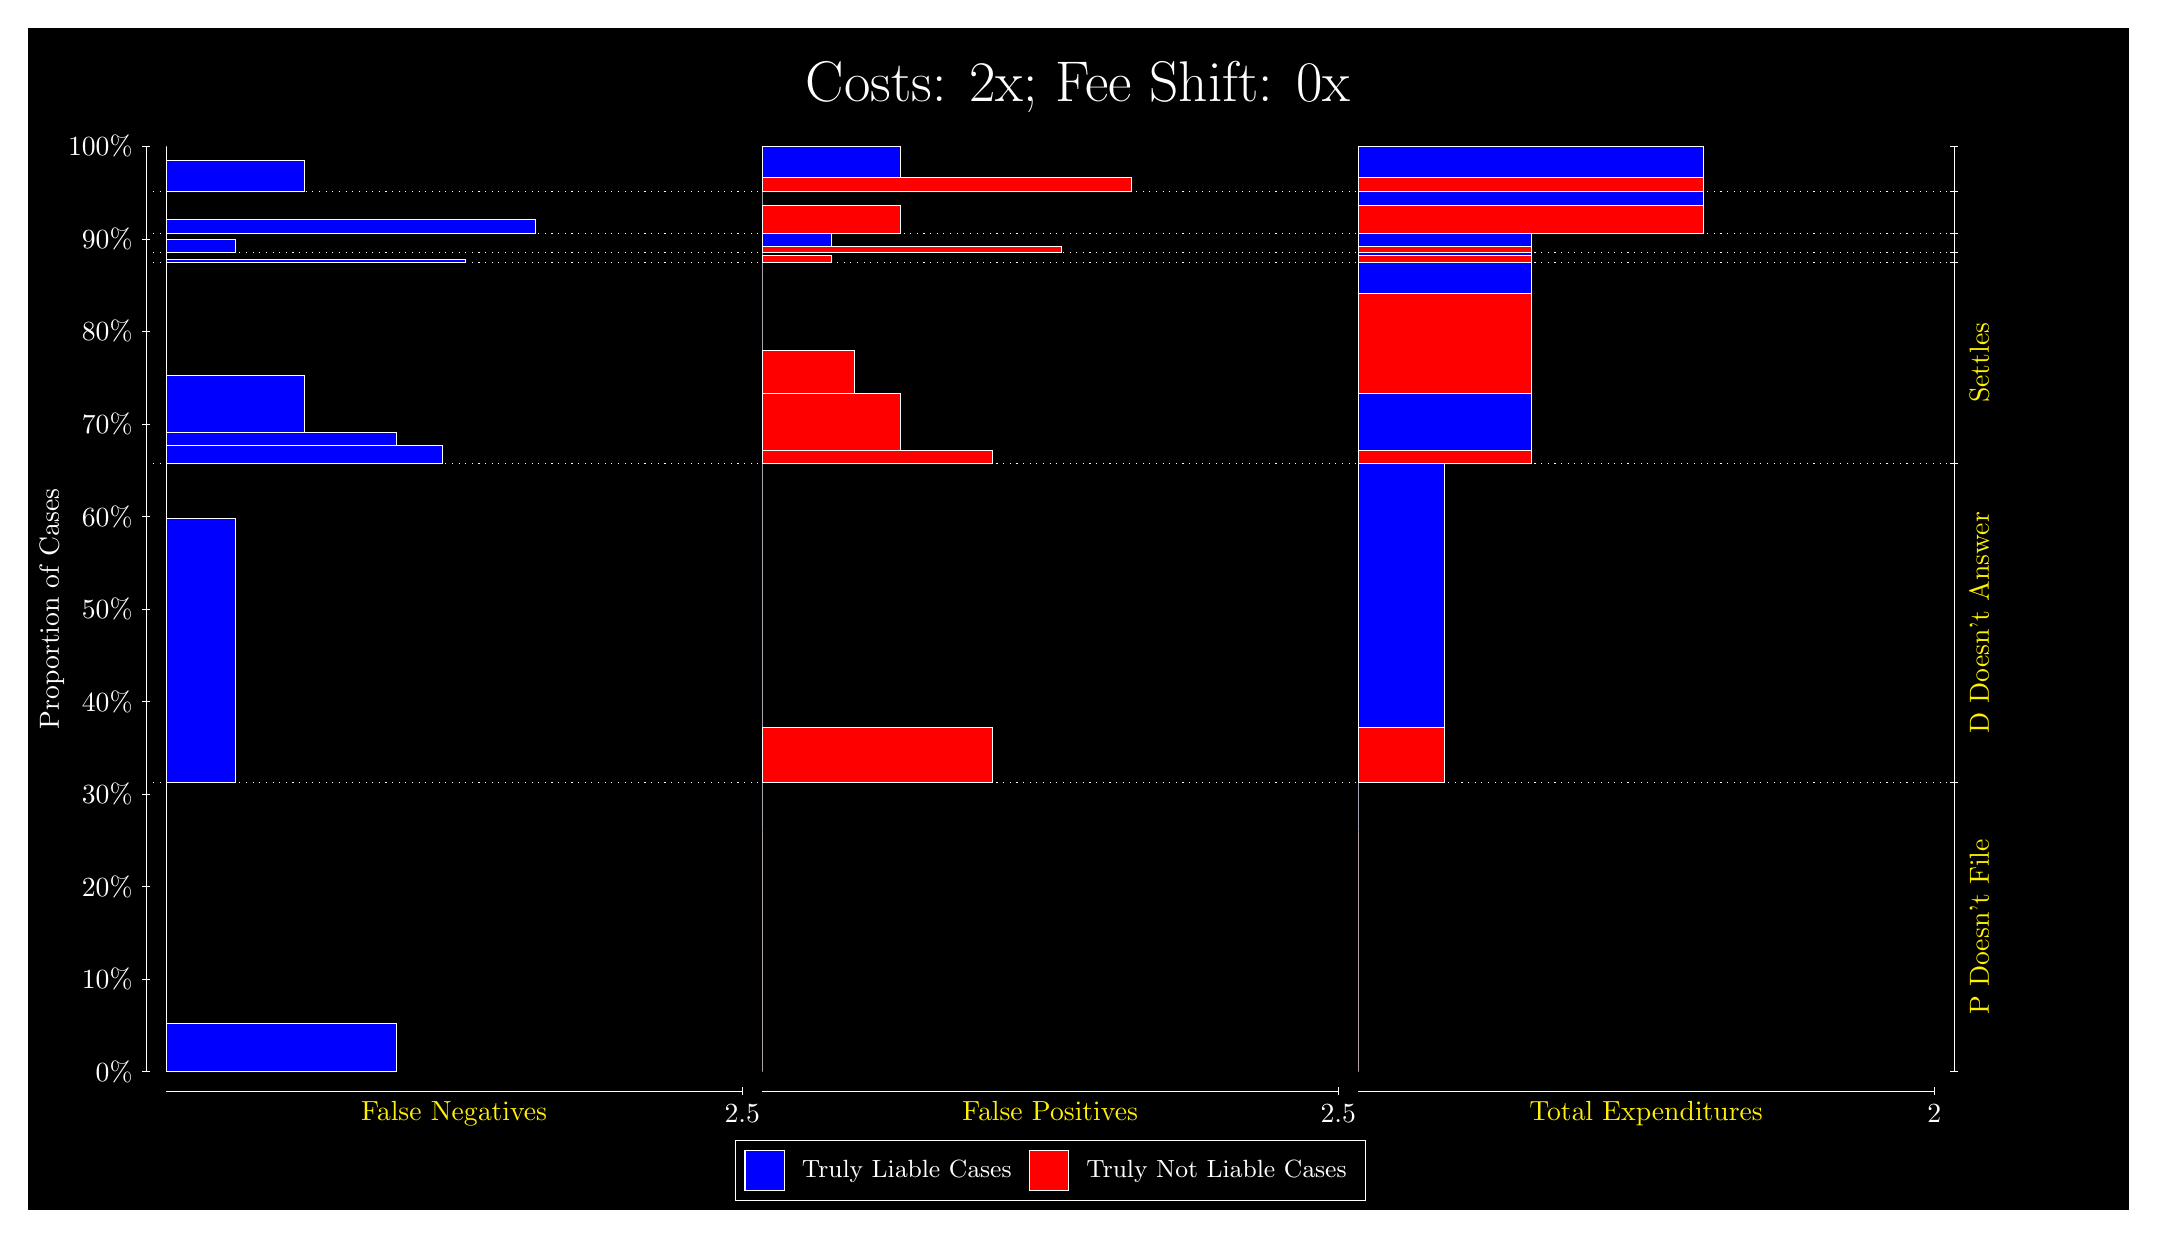
\begin{tikzpicture}
\draw[fill=black] (0,0) rectangle (26.667,15);
\draw[text=white] (0,13.5) rectangle (26.667,15) node[midway] {\huge Costs: 2x; Fee Shift: 0x};
\draw[white, very thin] (1.5,1.75) -- (1.5,13.5);
\node[rotate=90, text=white, anchor=center] at (0.3, 7.625) {Proportion of Cases};
\draw[white, very thin] (1.45,1.75) -- (1.55,1.75);
\node[text=white, anchor=east] at (1.45, 1.75) {0\%};
\draw[white, very thin] (1.45,2.925) -- (1.55,2.925);
\node[text=white, anchor=east] at (1.45, 2.925) {10\%};
\draw[white, very thin] (1.45,4.1) -- (1.55,4.1);
\node[text=white, anchor=east] at (1.45, 4.1) {20\%};
\draw[white, very thin] (1.45,5.275) -- (1.55,5.275);
\node[text=white, anchor=east] at (1.45, 5.275) {30\%};
\draw[white, very thin] (1.45,6.45) -- (1.55,6.45);
\node[text=white, anchor=east] at (1.45, 6.45) {40\%};
\draw[white, very thin] (1.45,7.625) -- (1.55,7.625);
\node[text=white, anchor=east] at (1.45, 7.625) {50\%};
\draw[white, very thin] (1.45,8.8) -- (1.55,8.8);
\node[text=white, anchor=east] at (1.45, 8.8) {60\%};
\draw[white, very thin] (1.45,9.975) -- (1.55,9.975);
\node[text=white, anchor=east] at (1.45, 9.975) {70\%};
\draw[white, very thin] (1.45,11.15) -- (1.55,11.15);
\node[text=white, anchor=east] at (1.45, 11.15) {80\%};
\draw[white, very thin] (1.45,12.325) -- (1.55,12.325);
\node[text=white, anchor=east] at (1.45, 12.325) {90\%};
\draw[white, very thin] (1.45,13.5) -- (1.55,13.5);
\node[text=white, anchor=east] at (1.45, 13.5) {100\%};

\draw[white, very thin] (24.457,1.75) -- (24.457,13.5);
\draw[white, very thin] (24.407,1.75) -- (24.507,1.75);
\node[anchor=west] at (24.407, 1.75) {};
\draw[white, very thin] (24.407,5.4196) -- (24.507,5.4196);
\node[anchor=west] at (24.407, 5.4196) {};
\draw[white, very thin] (24.407,9.4768) -- (24.507,9.4768);
\node[anchor=west] at (24.407, 9.4768) {};
\draw[white, very thin] (24.407,12.027) -- (24.507,12.027);
\node[anchor=west] at (24.407, 12.027) {};
\draw[white, very thin] (24.407,12.153) -- (24.507,12.153);
\node[anchor=west] at (24.407, 12.153) {};
\draw[white, very thin] (24.407,12.398) -- (24.507,12.398);
\node[anchor=west] at (24.407, 12.398) {};
\draw[white, very thin] (24.407,12.928) -- (24.507,12.928);
\node[anchor=west] at (24.407, 12.928) {};
\draw[white, very thin] (24.407,13.5) -- (24.507,13.5);
\node[anchor=west] at (24.407, 13.5) {};

\draw[white, very thin, fill=blue] (1.75,1.75) rectangle (4.6775,2.368);
\draw[white, very thin, fill=red] (1.75,2.368) rectangle (1.75,5.4196);
\draw[white, very thin, fill=blue] (1.75,5.4196) rectangle (2.6283,8.7805);
\draw[white, very thin, fill=red] (1.75,8.7805) rectangle (1.75,9.4768);
\draw[white, very thin, fill=blue] (1.75,9.4768) rectangle (5.2631,9.706);
\draw[white, very thin, fill=blue] (1.75,9.706) rectangle (4.6775,9.8683);
\draw[white, very thin, fill=blue] (1.75,9.8683) rectangle (3.5065,10.592);
\draw[white, very thin, fill=red] (1.75,10.592) rectangle (1.75,12.027);
\draw[white, very thin, fill=blue] (1.75,12.027) rectangle (5.5558,12.065);
\draw[white, very thin, fill=red] (1.75,12.065) rectangle (1.75,12.153);
\draw[white, very thin, fill=blue] (1.75,12.153) rectangle (2.6283,12.324);
\draw[white, very thin, fill=red] (1.75,12.324) rectangle (1.75,12.398);
\draw[white, very thin, fill=blue] (1.75,12.398) rectangle (6.4341,12.573);
\draw[white, very thin, fill=red] (1.75,12.573) rectangle (1.75,12.928);
\draw[white, very thin, fill=blue] (1.75,12.928) rectangle (3.5065,13.324);
\draw[white, very thin, fill=red] (1.75,13.324) rectangle (1.75,13.5);
\draw[white, very thin, fill=red] (9.3189,1.75) rectangle (9.3189,4.8015);
\draw[white, very thin, fill=blue] (9.3189,4.8015) rectangle (9.3189,5.4196);
\draw[white, very thin, fill=red] (9.3189,5.4196) rectangle (12.246,6.1159);
\draw[white, very thin, fill=blue] (9.3189,6.1159) rectangle (9.3189,9.4768);
\draw[white, very thin, fill=red] (9.3189,9.4768) rectangle (12.246,9.6391);
\draw[white, very thin, fill=red] (9.3189,9.6391) rectangle (11.075,10.363);
\draw[white, very thin, fill=red] (9.3189,10.363) rectangle (10.49,10.912);
\draw[white, very thin, fill=blue] (9.3189,10.912) rectangle (9.3189,12.027);
\draw[white, very thin, fill=red] (9.3189,12.027) rectangle (10.197,12.115);
\draw[white, very thin, fill=blue] (9.3189,12.115) rectangle (9.3189,12.153);
\draw[white, very thin, fill=red] (9.3189,12.153) rectangle (13.125,12.227);
\draw[white, very thin, fill=blue] (9.3189,12.227) rectangle (10.197,12.398);
\draw[white, very thin, fill=red] (9.3189,12.398) rectangle (11.075,12.752);
\draw[white, very thin, fill=blue] (9.3189,12.752) rectangle (9.3189,12.928);
\draw[white, very thin, fill=red] (9.3189,12.928) rectangle (14.003,13.104);
\draw[white, very thin, fill=blue] (9.3189,13.104) rectangle (11.075,13.5);
\draw[white, very thin, fill=red] (16.888,1.75) rectangle (16.888,4.8015);
\draw[white, very thin, fill=blue] (16.888,4.8015) rectangle (16.888,5.4196);
\draw[white, very thin, fill=red] (16.888,5.4196) rectangle (17.986,6.1159);
\draw[white, very thin, fill=blue] (16.888,6.1159) rectangle (17.986,9.4768);
\draw[white, very thin, fill=red] (16.888,9.4768) rectangle (19.083,9.6391);
\draw[white, very thin, fill=blue] (16.888,9.6391) rectangle (19.083,10.363);
\draw[white, very thin, fill=red] (16.888,10.363) rectangle (19.083,11.636);
\draw[white, very thin, fill=blue] (16.888,11.636) rectangle (19.083,12.027);
\draw[white, very thin, fill=red] (16.888,12.027) rectangle (19.083,12.115);
\draw[white, very thin, fill=blue] (16.888,12.115) rectangle (19.083,12.153);
\draw[white, very thin, fill=red] (16.888,12.153) rectangle (19.083,12.227);
\draw[white, very thin, fill=blue] (16.888,12.227) rectangle (19.083,12.398);
\draw[white, very thin, fill=red] (16.888,12.398) rectangle (21.279,12.752);
\draw[white, very thin, fill=blue] (16.888,12.752) rectangle (21.279,12.928);
\draw[white, very thin, fill=red] (16.888,12.928) rectangle (21.279,13.104);
\draw[white, very thin, fill=blue] (16.888,13.104) rectangle (21.279,13.5);
\draw[white, dotted] (1.5,5.4196) -- (24.457,5.4196);
\draw[white, dotted] (1.5,9.4768) -- (24.457,9.4768);
\draw[white, dotted] (1.5,12.027) -- (24.457,12.027);
\draw[white, dotted] (1.5,12.153) -- (24.457,12.153);
\draw[white, dotted] (1.5,12.398) -- (24.457,12.398);
\draw[white, dotted] (1.5,12.928) -- (24.457,12.928);
\draw[white, very thin] (1.75,1.5) -- (9.0689,1.5);
\node[text=yellow, anchor=north] at (5.4094, 1.5) {False Negatives};
\draw[white, very thin] (9.0689,1.45) -- (9.0689,1.55);
\node[text=white, anchor=north] at (9.0689, 1.45) {2.5};

\draw[white, very thin] (9.3189,1.5) -- (16.638,1.5);
\node[text=yellow, anchor=north] at (12.978, 1.5) {False Positives};
\draw[white, very thin] (16.638,1.45) -- (16.638,1.55);
\node[text=white, anchor=north] at (16.638, 1.45) {2.5};

\draw[white, very thin] (16.888,1.5) -- (24.207,1.5);
\node[text=yellow, anchor=north] at (20.547, 1.5) {Total Expenditures};
\draw[white, very thin] (24.207,1.45) -- (24.207,1.55);
\node[text=white, anchor=north] at (24.207, 1.45) {2};

\node[text=yellow, centered, rotate=90] at (24.777, 3.5848) {P Doesn't File};
\node[text=yellow, centered, rotate=90] at (24.777, 7.4482) {D Doesn't Answer};
\node[text=yellow, centered, rotate=90] at (24.777, 10.752) {Settles};





\draw (12.978300999999998,1.5) node[draw=none] (baseCoordinate) {};
\begin{scope}[align=center]
        \matrix[scale=0.5, draw=white, below=0.5cm of baseCoordinate, nodes={draw}, column sep=0.1cm]{
            \node[rectangle, draw, minimum width=0.5cm, minimum height=0.5cm, fill=blue] {}; &
            \node[draw=none, font=\small, text=white] (B) {Truly Liable Cases}; &
            \node[rectangle, draw, minimum width=0.5cm, minimum height=0.5cm, fill=red] {}; &
            \node[draw=none, font=\small, text=white] (B) {Truly Not Liable Cases}; \\
            };
\end{scope}

\end{tikzpicture}
\end{document}